\documentclass{article}
\usepackage[utf8]{inputenc}

\usepackage{amsmath}
\usepackage{amssymb}
\usepackage{graphicx}
\usepackage{tikz}
\usepackage{geometry}
 \geometry{
 a4paper,
 total={210mm,297mm},
 left=10mm,
 top=30mm,
 right=10mm
 }

\graphicspath{{./}}
\newcommand*\circled[1]{\tikz[baseline=(char.base)]{
    \node[shape=circle,draw,inner sep=0.5pt] (char) {#1};}}

\title{
\normalfont \large 
\textsc{Indian Institute of Technology, Ropar} \\    [40pt] 
\horrule{} \\[0.4cm] 
\Huge CS204 Course Project - Phase III\\ 
\horrule{} \\[0.5cm]
\protect\vspace{2.0cm}
\large
\textup{Team Members:}\\\vspace{1cm}
\begin{centering}
\begin{enumerate}
    \item Aditya Agarwal - 2019CSB1064
    \item Aneeket Mangal - 2019CSB1071
    \item Fadia Het Rakeshkumar - 2019CSB1084
    \item Shikhar Soni - 2019CSB1119
    \item Tanmay Aeron - 2019CSB1124
\end{enumerate}
\end{centering}
\date{}
\centering
\protect\vspace{4.0cm}

\includegraphics[width=1.0\textwidth]{riscv-logo-1.png}
}

\pagenumbering{roman}
\begin{document}
\maketitle
\newpage
\begin{centering}
\begin{Huge}
\textsf{Project Description}\\
\end{Huge}
\end{centering}
\protect\vspace{2.0cm}
\LARGE
The aim of this project is to simulate the machine level execution of RISC V 32-bit instructions using a high level language.\\

The Project also aims to give updates to the user regarding each step of the execution of the program. It also returns the final status of the memory and registers as output for the user to analyse the working of their programs thoroughly.\\

The Project currently allows the user to use 29 different instructions and can be extended to allow the use of any number of instructions by editing the .csv files as long as the instructions are supported by 32-bit RISC V ISA. \\

The program supports the use of `knobs' which will enable the user to select whether or not they want pipelining, data forwarding, and other details to be printed at the end of running the program.\\\\\\
The program executes each instruction using five stages as described in the RISC V architecture.\\
\newpage
There are 5 separate knobs, all with a different purpose.\\
\begin{enumerate}
  \item {\bf Knob1:} Used to enable/disable pipelining during runtime. 
  \item {\bf Knob2:} Used to enable/disable data forwarding
  \item {\bf Knob3:} Used to enable/disable printing values in the register file at the end of each cycle.
  \item {\bf Knob4:} Used to enable/disable printing information in the pipeline registers at the end of each cycle, along with the cycle number.
  \item {\bf Knob5:} This is like enabling knob4 for a specific instruction. We will be able to see pipeline register for that particular instruction only.
\end{enumerate}\\
The program also allows for the capability of a simple cache integrated with the previous phases of the project.\\
The cache is implemented using the concept of LRU(Least Recently Used) in which the data that was used least recently is deemed the victim block, and evicted from the cache.\\\\
There are two different caches:
\begin{enumerate}
    \item Instruction Cache (I\$)
    \item Data Cache (D\$)
\end{enumerate}\\
\vspace{1cm}All data during the Fetch stage is handled by the I\$ and all data during Memory Stage is handled by the D\$.\\

\newpage
\begin{centering}
\begin{Huge}
\begin{bf}
\vspace{2.0cm}
\textsf{Technologies employed}\\
\end{bf}
\end{Huge}
\end{centering}
\protect\vspace{2.0cm}
\textbf{}
\huge
Back-end - Python3
\begin{enumerate}
  \item {\bf pandas} for reading {\bf .csv} files.
  \item {\bf os} for getting and adding path to certain file locations.
  \item {\bf collections.defaultdict} to make a hash map for memory.
  \item {\bf sys} for reading and editing files with ease.
  \item {\bf json} for crunching data
\end{enumerate}\\
\textbf{}

Front-end - Python3
\begin{enumerate}
  \item {\bf PyQt5} for the Graphic User Interface.
  \item {\bf qdarkstyle} for dark theme in the GUI.
\end{enumerate}
\newpage
\textsl{\textbf{How to run the code:}}\\\\
\textsf{Instructions to run GUI version:}\\
\textsl{python main.py -g}\\
After running this command in the terminal, the GUI will pop up.\\
You can then enable each knob by ticking the checkbox for each.\\
For the fifth knob you can add the instruction number by adding the instruction in the box.\\
Information about the Fetch, Decode, etc. can be seen in the info tab on the right side when you click on the respective buttons in the DataPath tab
\par\noindent\rule{\textwidth}{0.4pt}
\textsf{Instructions to run Non GUI version:}\\
add `-k1' to enable knob1\\
add `-k2' to enable knob2\\
add `-k3' to enable knob3\\
add `-k4' to enable knob4\\
add `-k5 instruction number' to enable for that particular instruction\\
add `-ICache cachesize blocksize ways' for setting instruction cache details\\
add `-DCache cachesize blocksize ways' for setting data cache \\details\\
If you want to run a particular file, add that file in test folder and add `-f filename', otherwise main.mc is run\\
For example, if you want to enable knob1, knob2 , knob3, knob4 and knob5 with instruction 3, and make a data cache of size 512, block size 8 and ways to be equal to 2, and run fib.mc, write\\
\textsl{python main.py -k1 -k2 -k3 -k4 -k5 3 -DCache 512 8 2 -f fib.mc}\\
\newpage
\noindent
\textsf{Other features:}\\
\\
Arguments: [-h] [-g] [-f F] [-k1] [-k2] [-k3] [-k4] [-k5 INS] [-ICache cacheSize blockSize noOfWays] [-DCache cacheSize blockSize noOfWays]\\\\
\textsf{Description:}\\

\begin{enumerate}

  \item {[-h, -help]}        show help message and exit
  \item {[-g, -gui]}           enable GUI
  \item {[-f F, -filename F]}  specify file which is to be run, defaults to main.mc
  \item {[-k1, -knob1]}        enable Pipelining
  \item {[-k2, -knob2]}        enable Data Forwarding
  \item {[-k3, -knob3]}        show value in registerFile at end of each cycle
  \item {[-k4, -knob4]}        show value in Pipeline Registers at end of each cycle
  \item {[-k5 INS, -knob5 INS]}  show value in Pipeline Registers at end of each cycle for particular instruction
  \item {[ICache cacheSize blockSize noOfWays]} configure input cache in format cache size, block size and number of ways in Instruction Cache.
  \item {[DCache cacheSize blockSize noOfWays]} configure data cache in format cache size, block size and number of ways in Data Cache. If not specified both of the above default to 64 bytes (cache size), 4 bytes (block size), 2 (way set associative).
  \item {[-h]} for help on running the code
\end{enumerate}
\\
\newpage
\begin{centering}
\begin{Huge}
\textsf{Implementation Details}\\
\end{Huge}
\end{centering}
\protect\vspace{1.0cm}
We have implemented the project using the following method:\\

First it takes the input from a \textsl{\textbf{.mc}} file that contains the input in the required format, the content of this file can be modified using the GUI editor or by changing the main.mc file.\\
Then, it stores the \textsl{\textbf{.data}} part into the data memory and the \textsl{\textbf{.text}} part in the text part of the memory.
Once that is completed, we run the program using the following method:
\begin{enumerate}
\item Instruction Fetch: PC is incremented by 4, and the instruction is loaded from the memory and stored in the Instruction Register.
\item Instruction Decode: We are identifying the instruction using the .csv file and {\bf pandas} library and returning all the required fields. The registers RA and RB are also set during this stage.
\item Execute: The ALU executes the instruction by computing the desired output using values stored in registers in RA, RB, imm, etc. The required type of ALU instruction is determined by another .csv file. We are updating the output in the RZ register.
\item Memory Access: Memory is read and written in this stage. This stage is used only for load and store instructions. For the remaining instructions, this stage is redundant. The value of the RY register is also consequently updated.
\item Register Write-back: Here we are storing the value of the temporary register RY in the destination register, resulting in the register files being updated. The register update is extremely fast compared to memory read and update.
\end{enumerate}
\newpage
We have implemented data forwarding by passing the required values from the source buffer to the destination buffer without the need of stalling in most cases. This helps to reduce the number of stalls required. The types of data forwarding are:
\begin{enumerate}
    \item Execute to Execute
    \item Memory to Execute
    \item Memory to Memory
\end{enumerate}
\\
\vspace{1cm}

\vspace{1cm}\\
The program detects hazards present which can cause an incorrect value to be register due to one instruction's stage being executed before another. This is fixed by either transferring data values directly with the help of data forwarding, or with the help of stalling which delays the next instruction so that the previous one is updated in time.\\\\
While data forwarding is enabled, there is no use of stalling\\ except for one particular case where we use it along with \\Memory-to-Execute data forwarding.

\newpage
\begin{centering}
\begin{Huge}
\textsf{Input/Output format details}\\
\end{Huge}
\vspace{0.6cm}
\end{centering}
\noindent
\LARGE
{\bf Input Format:}\\\\
0x0 0x00500513\\
0x4 0x008000EF\\
0x8 0x0440006F\\
\$\\
0x10000000 0x64\\\\
The input is given through GUI if the GUI is run else it is taken from the input file.\\\\
The section given before the `\$' sign is the text segment of the code and all the lines after it signify the data segment of the code.\\\\
Output is generated in the `generated' folder. It contains the following things:  \\
\begin{enumerate}
    \item `registers.txt' contains the register values
    \item `memory.txt' contains the data part of the memory
    \item `stats.txt' contains the statistical details of the program
    \item `outputLog.txt' contains the buffer data of each cycle
    \item `buffer.txt' contains buffer data about the instruction given after k5 knob
    \item `CacheInfo.txt' contains information about the cache
    \item 'DataCache.txt' contains information about the data cache
    \item 'InstructionCache.txt' contains information about the instruction cache
    \item `forwarding.txt' contains information about forwarding used for front end information
    \item Buffer Snapshot and Register Snapshots folders are used for front end information
    
\end{enumerate}
\newpage
Example output for Buffer.txt\\\\
Fetch: (`00000000', `00400513', `00000004') \\
Decode: (9, `00000000', `00000000', `00000000', `00000000', 10, 0, 4, `00000004', `00000004', [[False, `NO', 0], [False, `NO', 0]]) \\
Execute: (9, `00000004', 10, `00000000', 0, 4, `00000004', `00000000') \\
MemoryAccess: (9, `00000004', 10, `00000000') \\\\
Example output for Forwarding.txt\\
{``EE1": ``F", ``EE2": ``F", ``ME1": ``F", ``ME2": ``F", ``MM": ``F"}\\
Here EE1:F means forwarding of Execute to Execute between prev instruction(1 means previous instruction) and current instruction is False\\
Similarly ME2: T means forwarding from Memory to Execute from previous to previous instruction(2 means previous to previous instruction) is True\\\\
CacheInfo.txt\\
`F' stands for Fetch, `L' stands for Load and `S' stands for Store\\
In the Cache Info in Fetch the index, Set, isMiss and Victim block is printed\\
Here the isMiss = T means isMiss is True and so we found a miss\\
Similarly if Fetch or Load or Store is -1 means the corresponding instruction is not executed.\\
\\The user can specify input configurations for the Instruction Cache and Data Cache separately. Outputs for the two will also be displayed separately.\\
Input parameters that can be set by the user include:
\begin{enumerate}
    \item Cache size
    \item Cache Block size
    \item Number of ways for Set Associative
\end{enumerate}
\\Output parameters include:
\begin{enumerate}
    \item Number of accesses
    \item Number of hits
    \item Number of misses
\end{enumerate}

\newpage
\Large
\textbf{In \textsl{stats.txt} we have printed the following:}

\begin{enumerate}
\begin{LARGE}
\item \textsf{Total number of cycles}
\item \textsf{Total number of instructions executed}
\item \textsf{CPI}
\item \textsf{Data Transfer instructions executed}
\item \textsf{ALU instructions executed}
\item \textsf{Control instructions executed}
\item \textsf{Total Stall Count}
\item \textsf{Number of Data Hazards}
\item \textsf{Total Control Hazards}
\item \textsf{Total Branch misprediction}
\item \textsf{Number of stalls due to data hazards}
\item \textsf{Number of stalls due to control hazards}
\end{LARGE}
\end{enumerate}

\par\noindent\rule{\textwidth}{0.4pt}



\noindent
\textbf{An example output for \textsl{stats.txt} is :}\\
\\
\begin{LARGE}
\textsf{Total number of Cycles in the program :14}\\
\textsf{Total number of Instructions executed :4}\\
\textsf{CPI is :3.5}\\
\textsf{Data Transfer Instructions Executed :0}\\
\textsf{ALU instructions are :4}\\
\textsf{Contol instructions :0}\\
\textsf{Total Stall Count are :6}\\
\textsf{Number of Data Hazards are :3}\\
\textsf{Total Control Hazards are :0}\\
\textsf{Total Branch mispredictions are :0}\\
\textsf{Number of stalls due to data hazards are :6}\\
\textsf{Number of stalls due to control hazards are :0}\\\\
\textsf{The instruction fed was:}\\
\textsf{0x0	0x00A50513}\\
\textsf{0x4	0x00A50513}\\
\textsf{0x8	0x00A50513}\\
\textsf{0xC	0x00A50513}\\
\end{LARGE}
\vspace{0.6cm}

\noindent
\newpage

\begin{Huge}
\centering{\textsf{Graphical User Interface}}\\
\end{Huge}
\vspace{2cm}
\begin{centering}
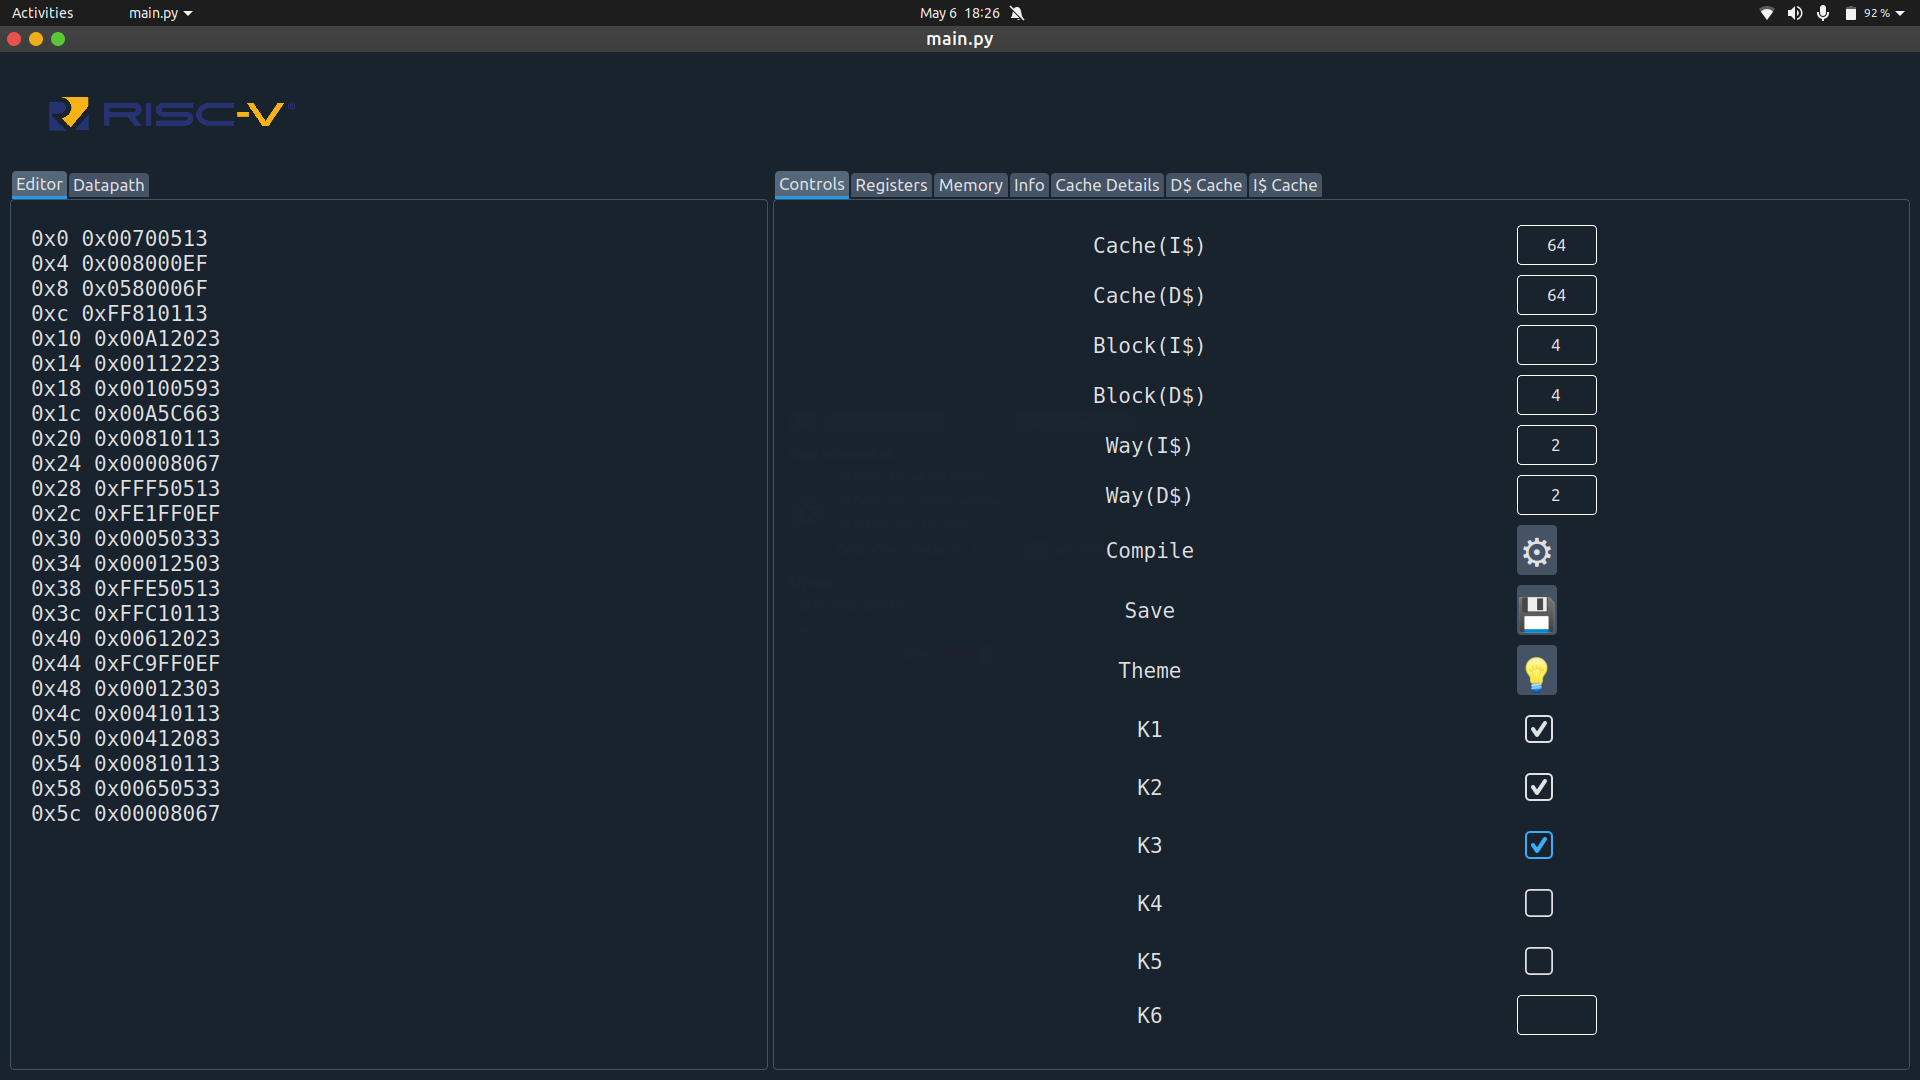
\includegraphics[width=1.0\textwidth]{controls.png}\vspace{2cm}
\end{centering}
Above is the GUI image, the tab on the right is the `controls tab' and the user can change the knobs and cache configurations accordingly (cache size must be greater than the block size and the cache size should be a power of 2  along with the block size being a multiple of 4 to ensure word alignment).\\
\unindent
We can input the Cache Size, Block Size (in bytes) and Ways on the right side of the page.\\
We can enable the knobs by ticking the corresponding boxes, for knob5 one needs to enter the instruction number on the 'k6' block (if no number is entered then it defaults to 1).
We can compile the code by pressing the `Settings/Compile' icon corresponding to compile, there's also the save icon below it represented by a `floppy disk'.\\
We can also change the theme by clicking the `bulb button' to change from light to dark mode and vice versa.
\unindent
When we press the compile button the code in the editor gets saved in main.mc and the code will be executed.
\newpage
\begin{centering}
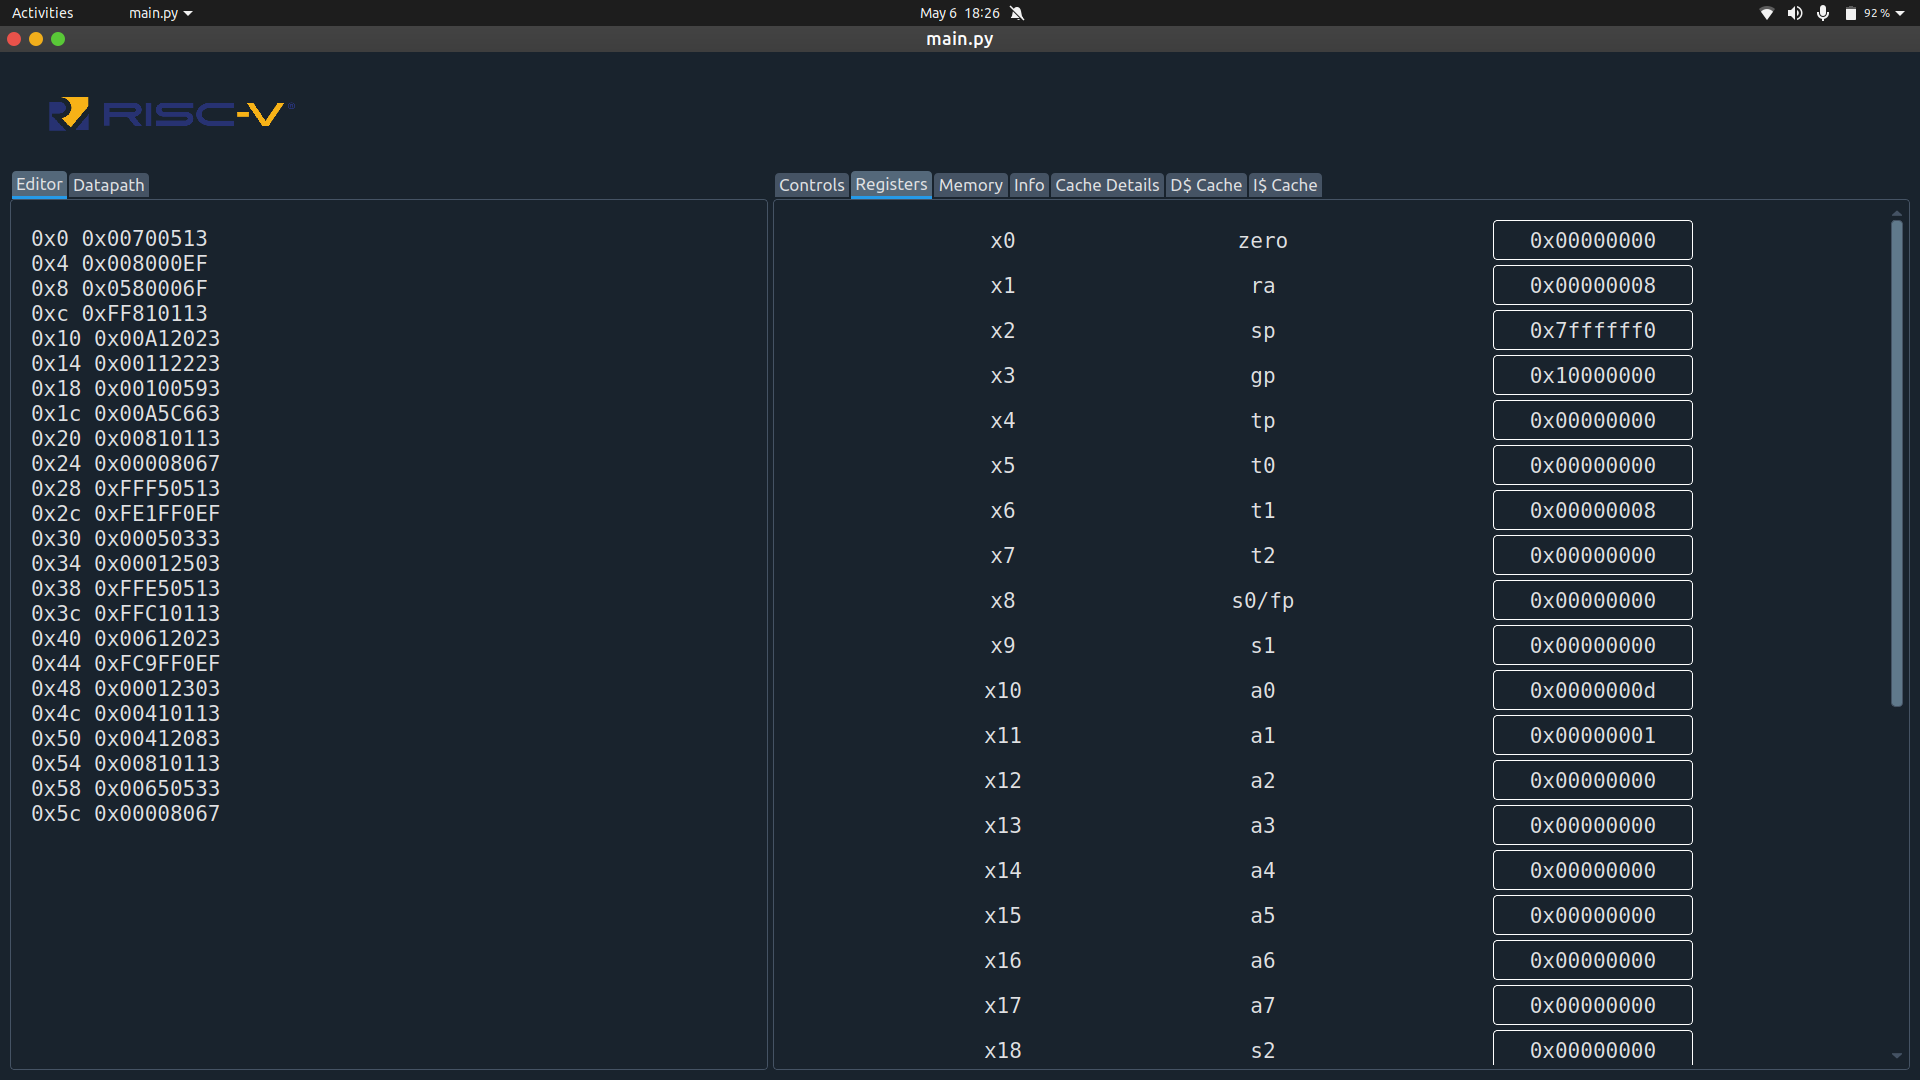
\includegraphics[width=1.0\textwidth]{registers.png}\vspace{2cm}
\end{centering}
We can see the values stored in all the Registers here. Values are stored in Hexadecimal format.\\
User can scroll down to observe the registers that are not immediately visible on the screen.


\newpage
\begin{centering}
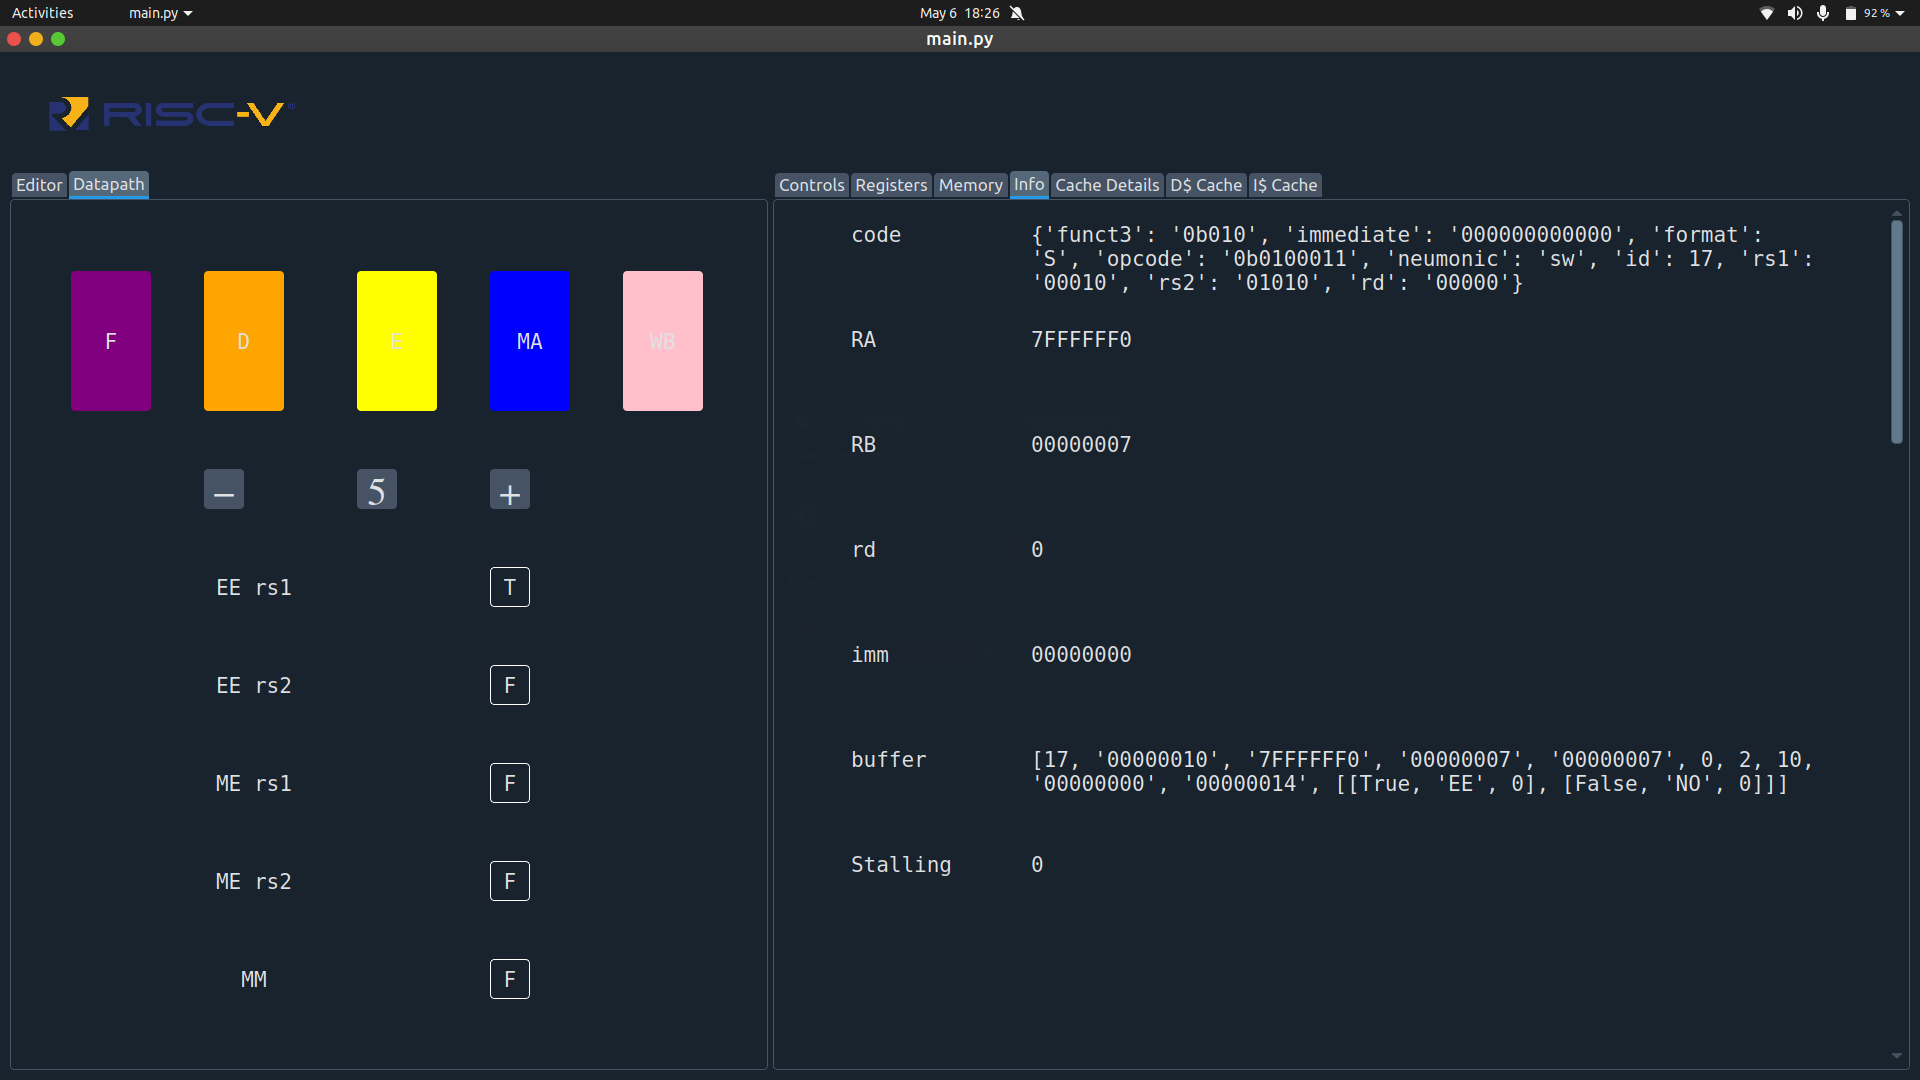
\includegraphics[width=1.0\textwidth]{info.png}\vspace{2cm}
\end{centering}
The `info tab' contains all the necessary information about the pipelined execution of each stage. It should only be used when the code is run in pipelined mode.\\
We can see the info about each cycle and each stage.
The cycle for which info is seen is seen in the box. In the image, we are checking details for the 5th cycle.\\
One can increase or decrease the total cycles by clicking '+' or '-' respectively. One can't change cycles beyond the total number of cycles of the program or less than 0 either.\\
We can see the info about the stage by clicking the `$F$' `$D$' `$E$' `$MA$' or `$WB$' boxes accordingly.\\
EE rs1 `T' implies that there is Execute to Execute forwarding going on because of a data hazard in rs1.

\newpage
\begin{centering}
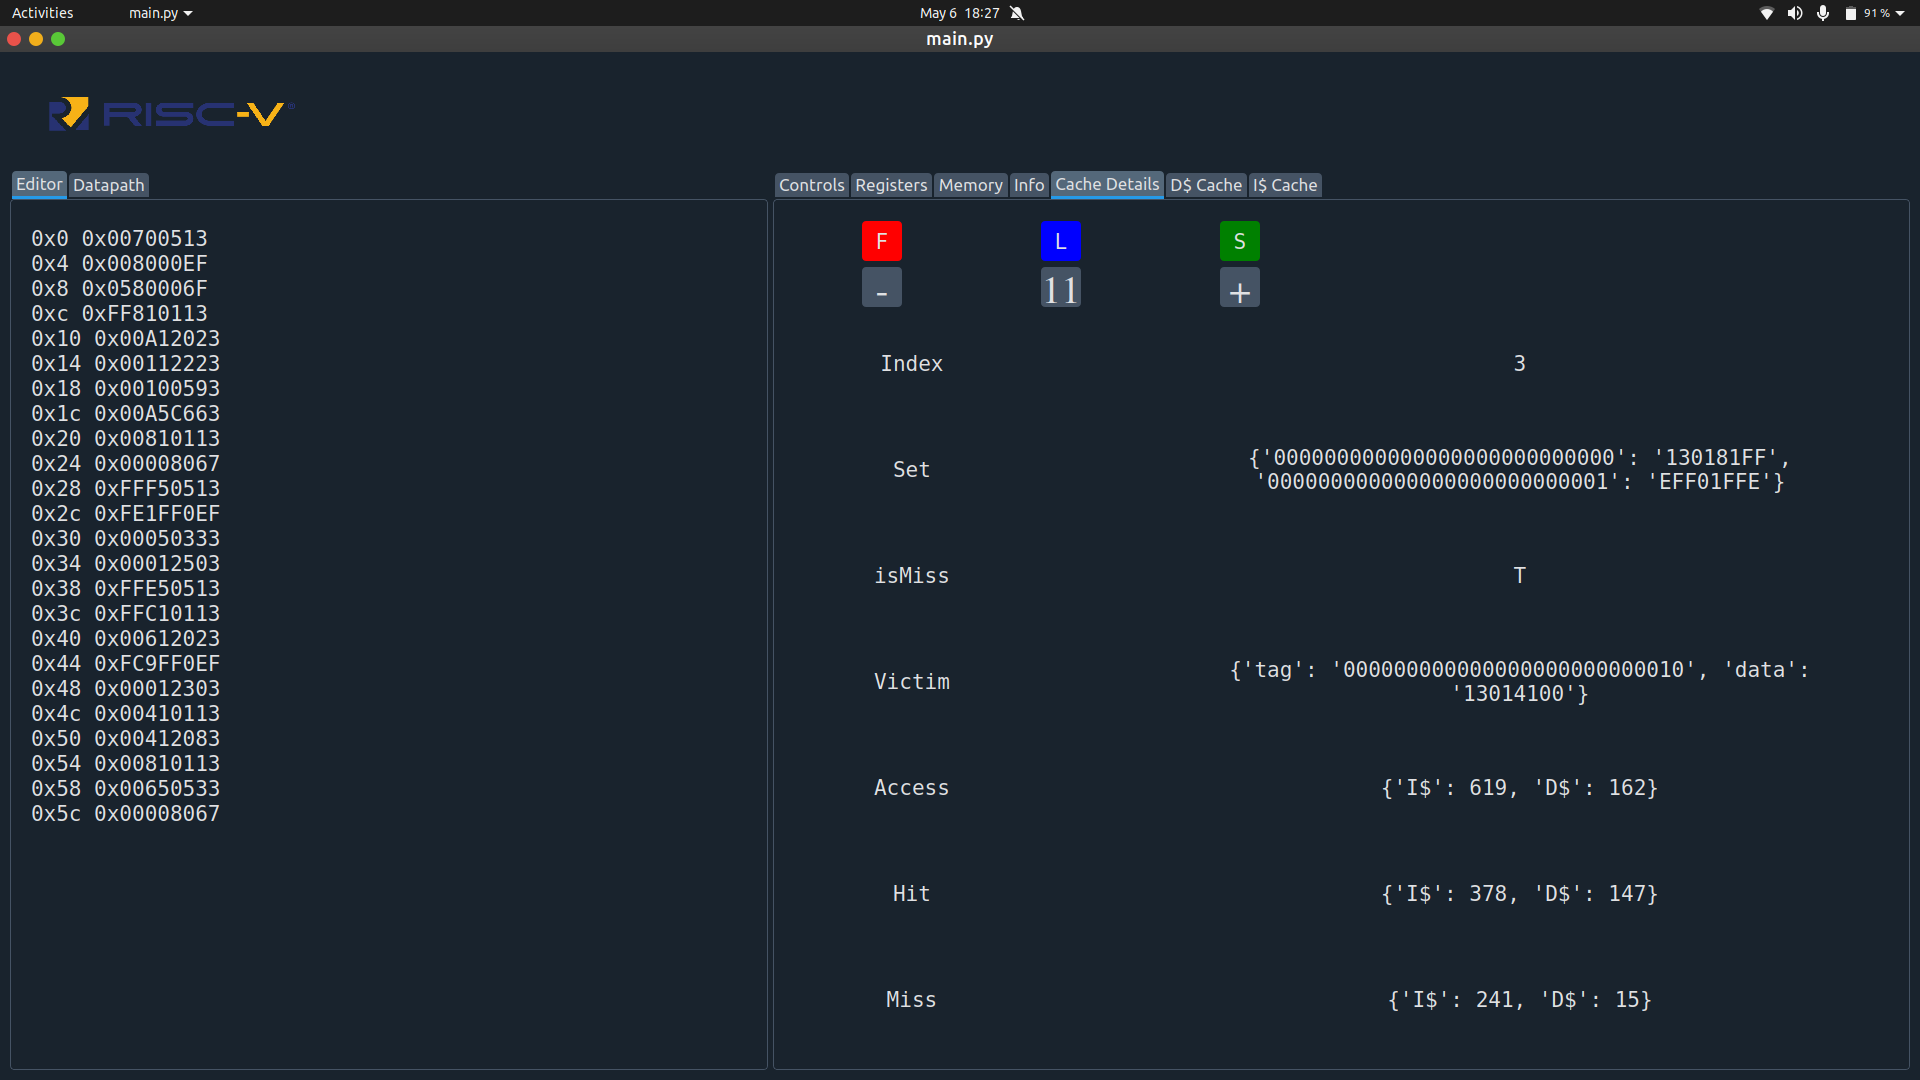
\includegraphics[width=1.0\textwidth]{cache_details.png}\vspace{2cm}
\end{centering}
We can see the Cache Details corresponding to the selected cycle.\\
One can increase or decrease the total cycles by clicking '+' or '-' respectively. One can't change cycles beyond the total number of cycles of the program or less than 0 either.\\
We can see the details about Fetch, Load, and Store accordingly by clicking on that block.\\
`isMiss' is T(meaning True) when Miss occurs else it is F(meaning False).
Here we can see the Total number of Accesses, Hits, Misses for Instruction and Data respectively, they are independent of the cycle number and are the net stats after the execution of the whole program.\\
The tag and data of the Victim is shown in the Victim block. If no data is present then it will be -1.\\
For example if you want to see the Load Cache Details for the 11th cycle first go to the 11th cycle and then click on the Load button.\\
\newpage

\vspace{2cm}
\begin{centering}
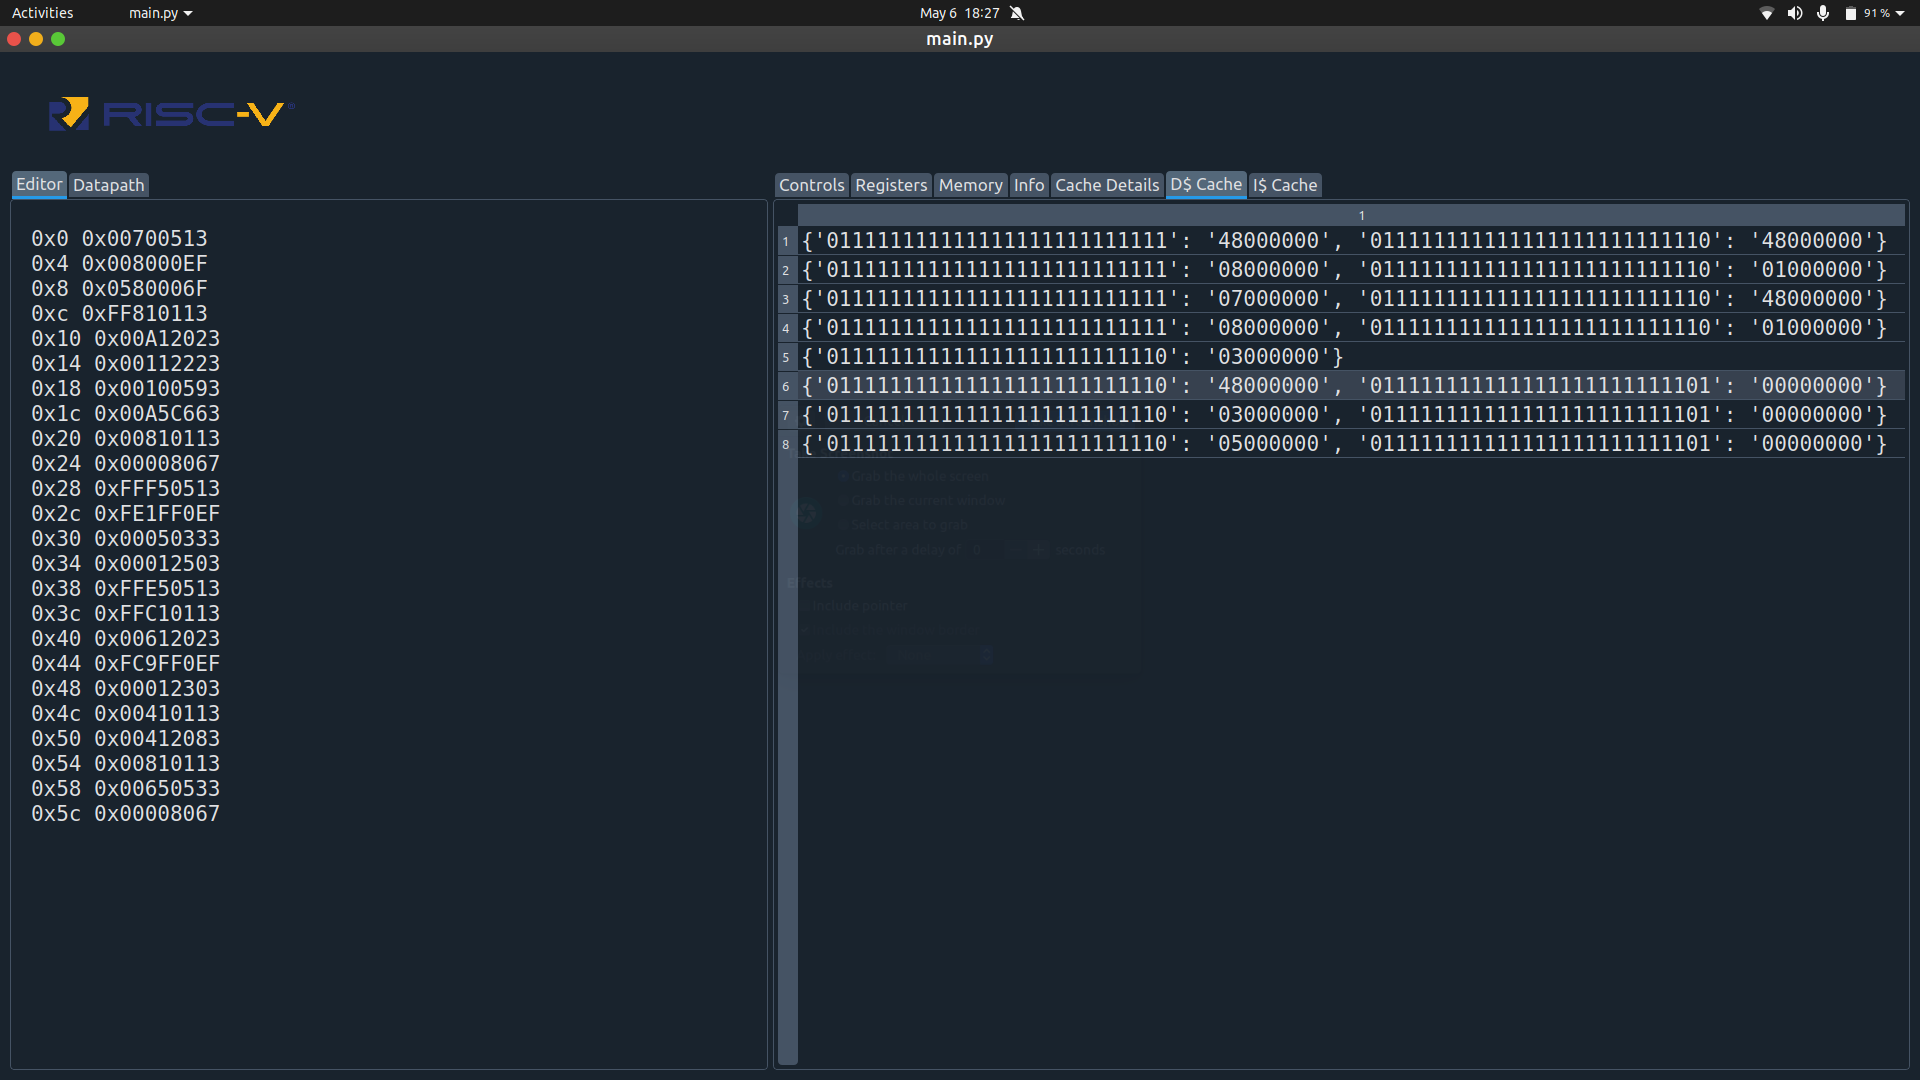
\includegraphics[width=1.0\textwidth]{data_cache.png}\vspace{2cm}
\end{centering}
The information about the Data Cache is seen here\\
We can see the whole info by double clicking on the corresponding box.
We can then scroll thorugh the info using the right or left arrow key.\\
One set is represented by the line number and the total blocks in it are given in a line. One block is of the format \{tag:``data"\}.\\

\newpage
\begin{centering}
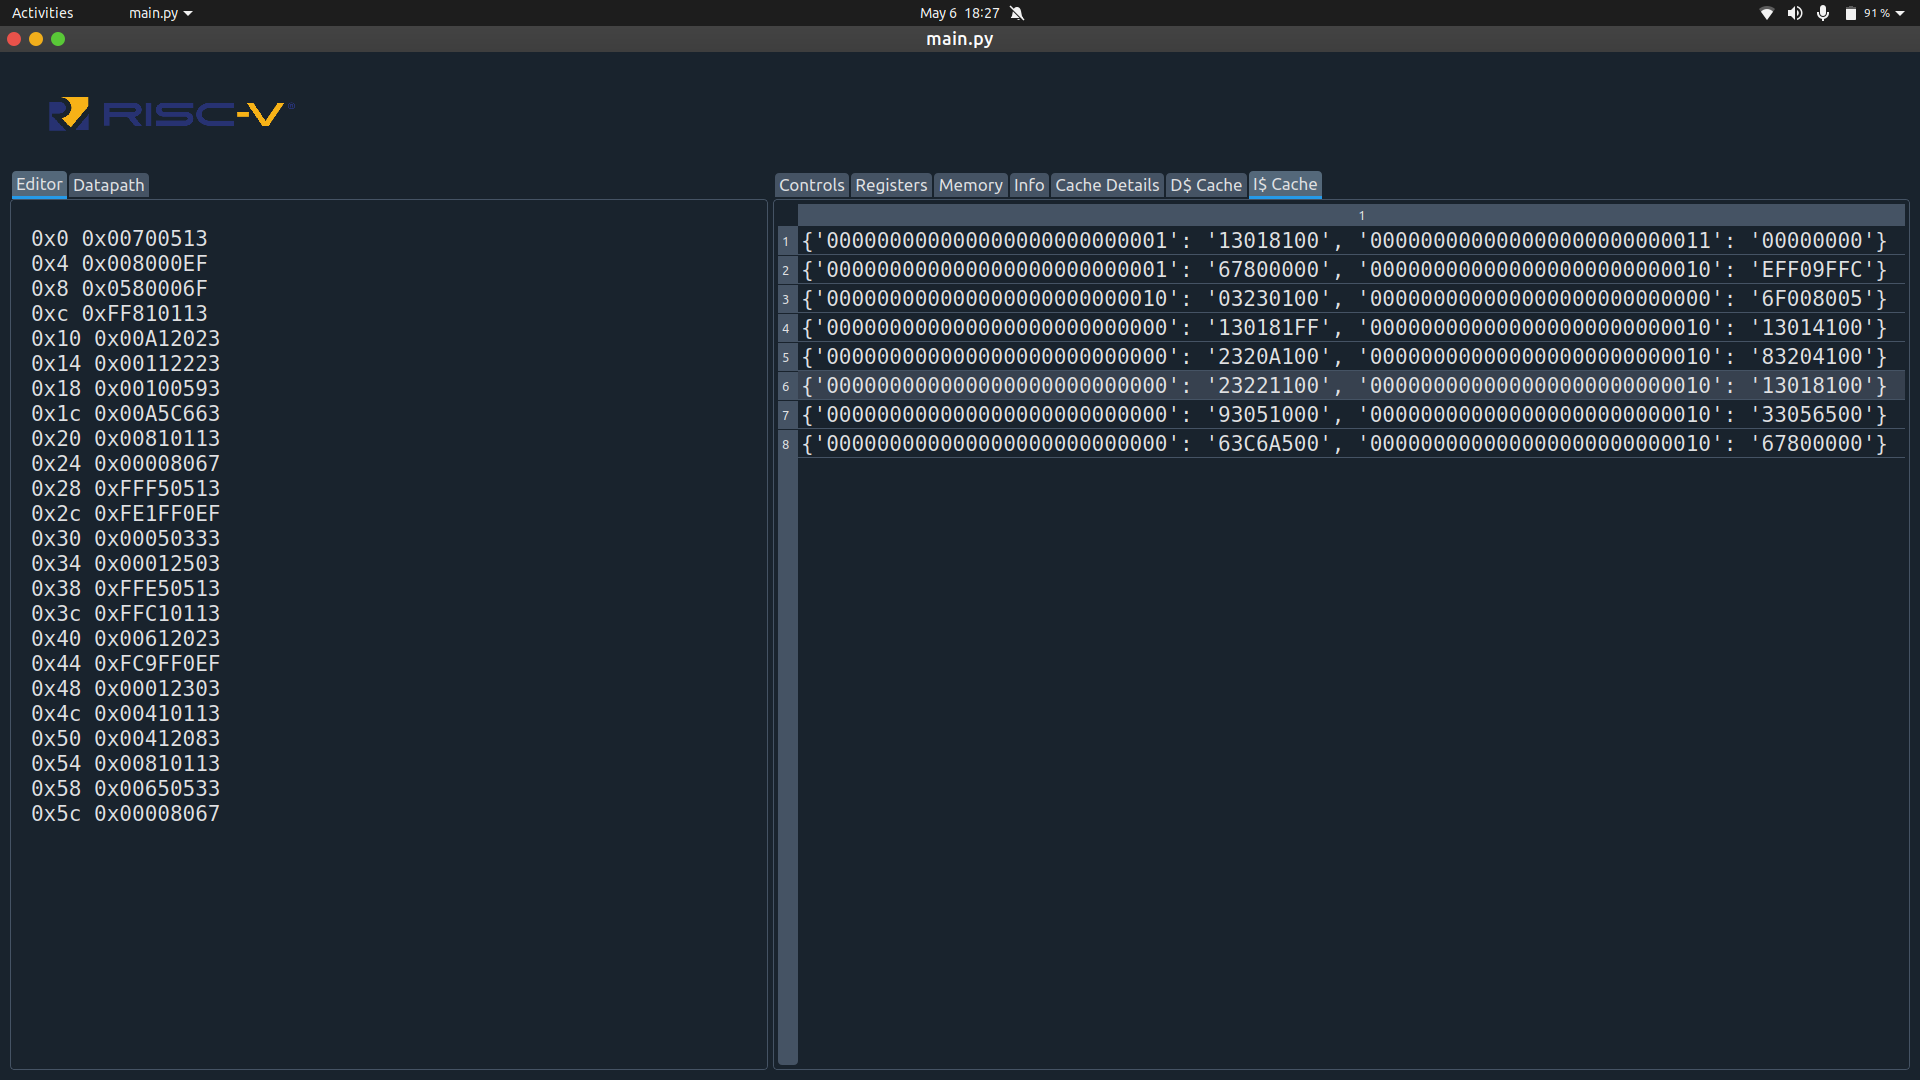
\includegraphics[width=1.0\textwidth]{ins_cache.png}\vspace{2cm}
\end{centering}
The information about the Data Cache is seen here\\
We can see the whole info by double clicking on the corresponding box.
We can then scroll thorugh the info using the right or left arrow key.\\
One set is represented by the line number and the total blocks in it are given in a line. One block is of the format \{tag:``data"\}.\\

\newpage

\vspace{4cm}

\newpage

\begin{centering}

\includegraphics[width=1.0\textwidth]{memory.png}\vspace{2cm}
\end{centering}
\\
\LARGE
In the memory we can see the address and the value at each address. \\
For example if the address is 0x1000000C then the address of each of the right box are 0x1000000C , 0x1000000D, 0x1000000E and 0x1000000F.\\
Here we can see the jump to register functionality, where we have stored a value in the register 0x10000500, and are jumping to it and seeing the value.\\
\unindent
For example to jump on the location 0x10000500 write `10000500' in the Jump to box which is in the bottom right in the memory tab.


\newpage
\def\checkmark{\tikz\fill[scale=0.4](0,.35) -- (.25,0) -- (1,.7) -- (.25,.15) -- cycle;}
\LARGE
\\\\
We have shown memory, registers and info on the right section of the GUI while on the left part there is Code Editor.\\
In the Code Editor you can edit your code or copy paste your code and also save it.\\
The info contains the details of the instruction being executed in each stage during a cycle.\\
First of all we will paste the code in the Editor on the left side and then save and compile the code by clicking the respective `save' button which is the first button on the top right and `compile' button. The code will get updated in \textsl{\textbf{main.mc}} file and then the code will be executed and a \checkmark\hspace{0.7mm} will appear. The memory and registers will be updated simultaneously.\\\\
\unindent
Other details are present in their respective tabs as described earlier.\\\\
\unindent
Refer to the next page for a more detailed explanation of each tab and it's purpose.\\

\newpage
\begin{centering}
\begin{Huge}
\textsf{Summary of the details of the layout of the GUI}\\
\end{Huge}
\vspace{0.6cm}
\end{centering}


\begin{itemize}
    \item We can jump to the memory using the `Jump to' box on the bottom right corner in the memory section.
    \item All the registers can be seen in the register file by scrolling in the register file section.
    \item Executing \textsl{\textbf{main.py}} always generates a GUI window where you can code in the Editor.
    \item We can also execute non GUI code by writing\textrightarrow   python main.py
    \item The DataPath explains how the data is flowing through each stage.
    \item Here the 5 stages can be seen in the DataPath tab.
    \item The number below it is the cycle number for which the DataPath is shown.
    \item You can see the DataPath in the respective cycle by going to that cycle.
    \item Click on + to go to the next cycle and on - to go to the previous cycle.
    \item We can observe all the required data in the cache by clicking on the required tabs
    \item One tab is meant to observe the Victim block in each cycle, where you can adjust the cycle number similar to the `datapath tab' along with the details of individual sets during that cycle.
    \item Two more tabs are there for observing the final state of the instruction cache (I\$) or data cache (D\$) respectively after the program has run.
\end{itemize}

\end{document}



